\chapter{Finger exercises} \label{chap:finger_exercises}

\section{Fretting hand}

\subsection{Play songs and scales slow}

By just practicing a song slow and with a metronome, you can focus on good finger placement. Focus on a clear sound of the note.

\subsection{Spider exercise}

There are many variations of the spider exercise. But \autoref{fig:guitar_spider_exercise} focuses on straight finger placement. If you don't have your fingers correct on the strings, you will mute the lower string, resulting in unclear notes when playing notes on that string.

\begin{figure}[h]
	\centering
	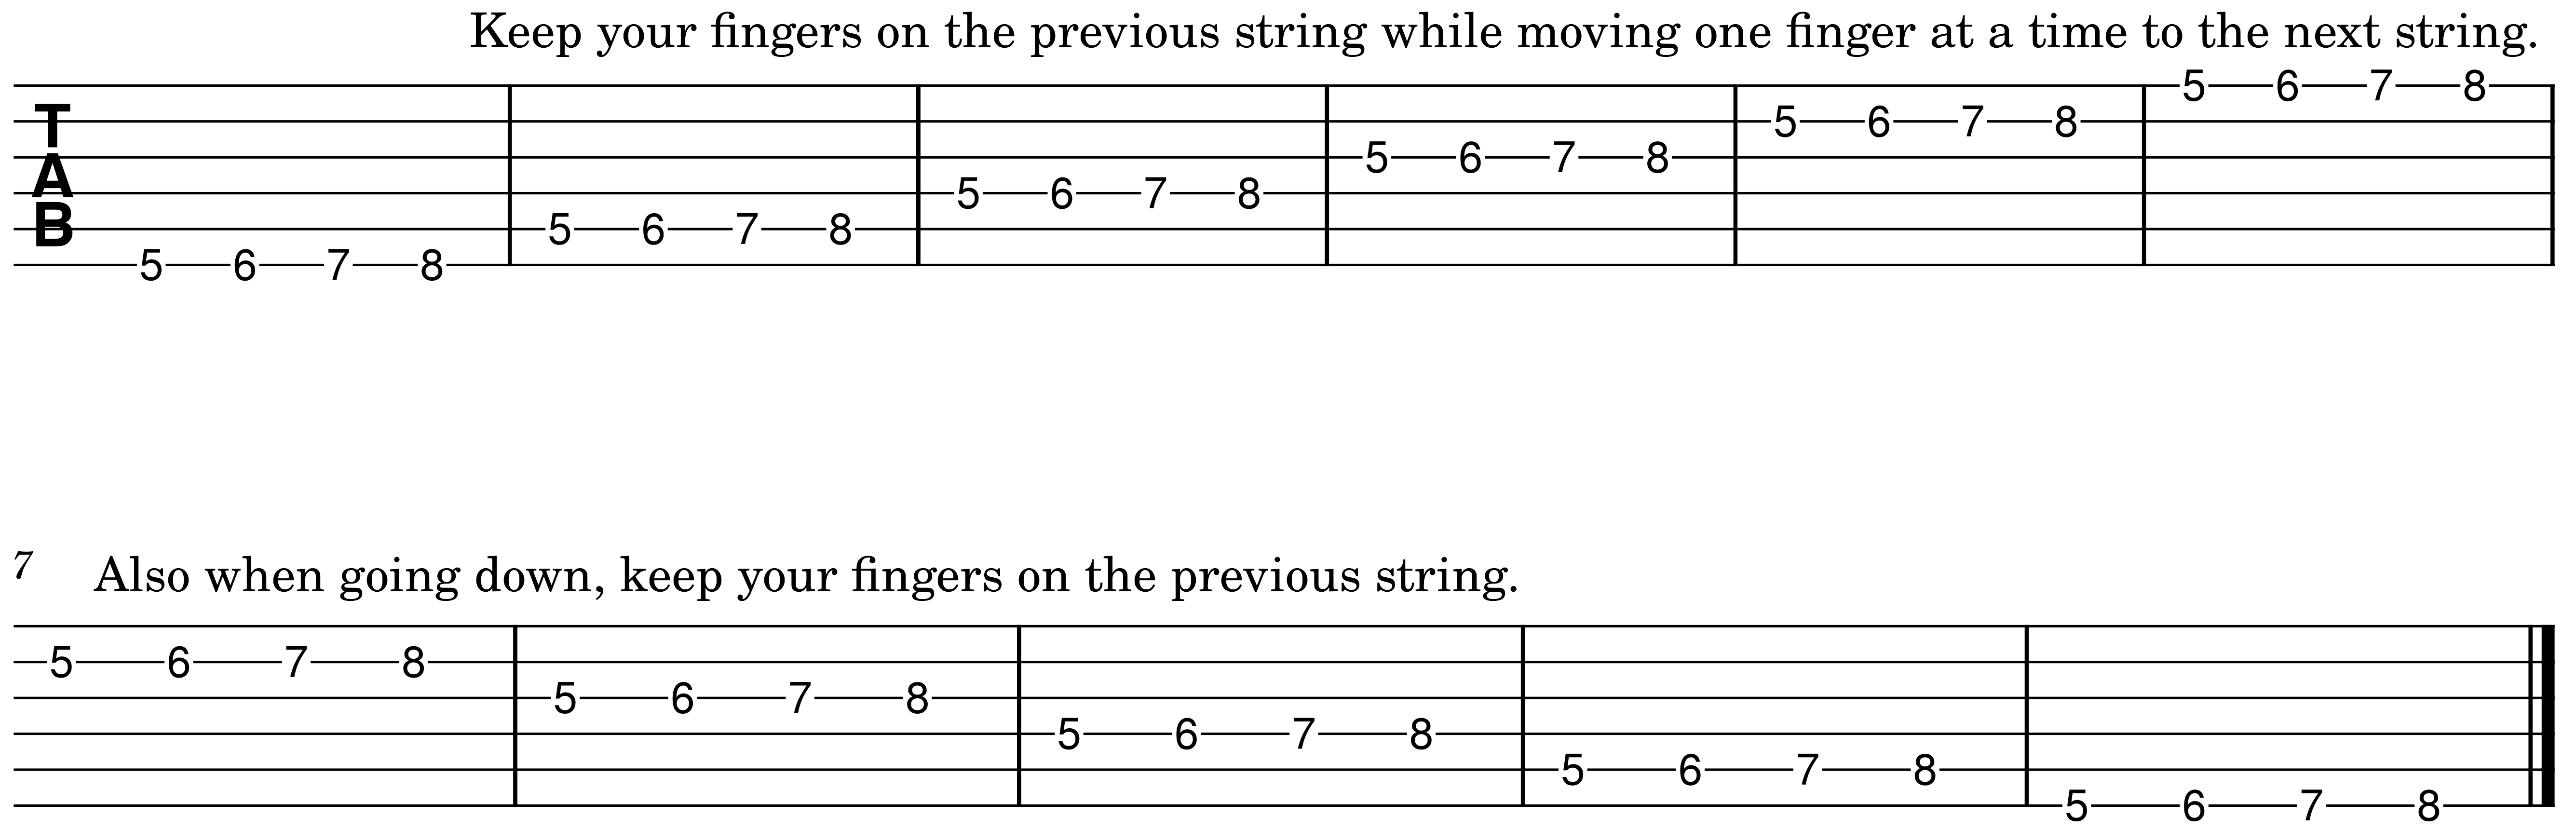
\includegraphics[width=\textwidth]{../../MuseScore/Guitar/guitar_basic_spider_exercise.png}
	\caption{Spider exercise}
	\label{fig:guitar_spider_exercise}
\end{figure}

You can of course start on a different fret than the 5th. And you could also for example skip each-other string. \autoref{fig:guitar_spider_exercise} is just the basis.

\section{Strumming \& picking hand}
TODO